\section{When dreams come true - The discovery of Karstaway} 
\begin{marginfigure}
\begin{tikzpicture}
\node [name-dest] (box){%
    \begin{minipage}{\textwidth}
     \begin{itemize}
    \item Jack Hare
    \item Tanguy Racine
    \end{itemize}
    \end{minipage}

};
\node[fancytitle, right=10pt] at (box.north west) {Karstaway};
\end{tikzpicture}
\end{marginfigure}

\begin{marginfigure}
\centering
\frame{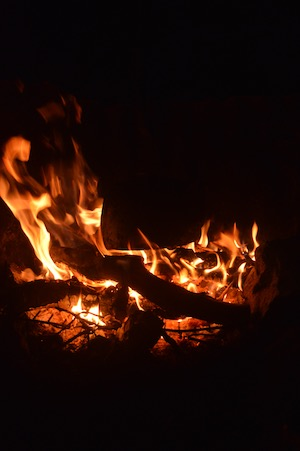
\includegraphics[width=\textwidth]{images/2016/tanguy-karstaway-2016/teapot-2016.jpg}}
\caption{The best caving plans are concocted next to a boiling kettle --- Tanguy Racine}
\label{teapot}
\end{marginfigure}

I was keen to go caving with Jack, not having the opportunity to do it in 2015. We'd put quite a bit of work into rigging the abseil to Primadona, and things were looking up in the Galerija branch of the cave. Memory of previous leads in this zone had not faded as much as for the rest of the cave, and after the first spark of exploration in Quantum State it was time I got some findings under the belt.

On the surface, we had a good plan: going in Galerija, and traversing at the top of Quantum state, we'd be able to reach a zone with several open leads (as shown by the 2011 survey). We only had one pitch to rerig on the way: the 20m hang dropping at the start of Smer0 and Galerija, which had been dubbed Knot So Great. There was an early start in the Bivi and early enough we reached said pitch. Bolts in, rope tied, descender rigged, I descended, placed a rebelay and frowned upon the rope rub that had appeared just on top of it. The old slov rope was within reach, tied to a rebelay two metres above mine. I grabbed the rope, cut it and tied a deviation. The bundle of rope dropped to the bottom. This done I went down, quickly finding myself under a small drip. 

The bottom of the pitch was a larger space, draughty and noisy, littered with sharp, shiny white boulders of all kinds of sizes. At the bottom, we were joined with Rhys and Will Scott who'd caught up with us and had a plan to push the stream underneath the same boulders. Jack and I pressed on in the windy Galerija, glancing at the floor and ceiling, looking for leads others might have missed. There was a tight, loose cobbly tube before Quantum State I popped my head into but thought better of it. Past Quantum state, gingerly, ever so gingerly Jack and I traversed over the pitch head, sending a few cobbles and blocks of mud down the black throat of the pitch. On the far side, new territory awaited: a rift, guided by a fault plane, with thick protrusions of white rock and a howling draught.

After a few twists, the floor dropped two metres, into a puddle of brown mud. We dropped that as Jack muttered ?Should be fun to climb back up'. There were a few tens of metres of meandering rift with a high way along the top of the rift, leading to committing crawl over boulders. We'd lost the draught there so opted for the lower way down, hugging the bottom of the rift, and following the gale. A few more drops, and around a corner a large yellow tacklesack. Beyond that, a rope led into the darkness of large pitch.

After a cursory inspection of the hangers and rope we decided it was okay to descend. The drop was a clean hang, perhaps 30m deep, in a pitch some ten metres in diameter. At the bottom a cairn had been built well out in the centre. Jack had been quickly scouting the ways onwards. It seemed we'd reached TTT, as this was what Zdenko thought likely. If it was, then the connection had not been marked on the survey. The way down was obvious but tricky. The first free-climb down was not very tricky, nor the second. The passage turned left, there was another down climb where the passage wall widened underneath the ledge we'd come to. There were plenty footholds, but I remarked ?Those free-climbs are looking more and more dubious'. 

\begin{figure*}[t!]
\centering
\frame{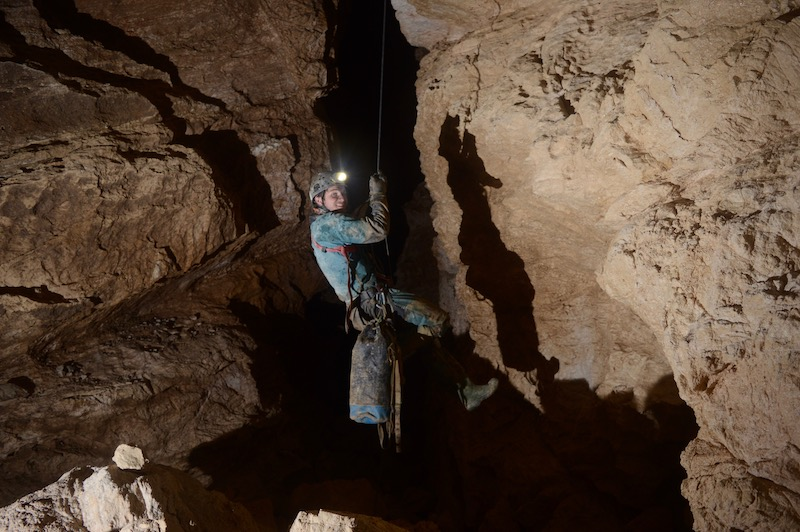
\includegraphics[width=\textwidth]{images/2016/tanguy-karstaway-2016/wills-2016.jpg}}
\caption{Will Scott ascending Rokovo Brezno, the 30m pitch--- Tanguy Racine}
\label{Rokovobrezno}
\end{figure*}

Jack took over the lead for the next drop, which was frankly terrifying: traversing around a ledge, hands on the opposite wall till the walls got far enough together that we could bridge down. At the bottom we considered what we just did, with doubts gnawing at us: surely this should have been rigged? Upon inspection, the way on didn't bear any footprints, nor any other sign of previous discovery. We were then almost certain what we found next was virgin passage and the way on looked promising: wide, with a small stream and a howling draught.

At the bottom of the down climb was as good a spot as any to have a lunch break, and the cheese and fish we'd brought down made for a very welcome fare. Without delay Jack led the way into the streamway. For two metres it was storming. After that, it degenerated into a tight rift, with a large, pointy boulder providing the chief obstacle to easy progress. The passage went on nonetheless, and what's more the loud splashing of a waterfall could be heard further on. After a short way, the width of the passage increased, and we saw the water, went past it to reach a ten metre aven chamber where the direction of the passage veered into the west. A small series of scalloped passages led to a white dry twisting rift. The water plunged somewhere underneath, but we preferred the wider, upper level dry passage, which continued to a pitch head. The rift itself was very white, with a white clay to silt draping the knocks and crannies of the walls. Within this matrix there were larger granules of haematite, no bigger than a couple millimetres. 

\begin{marginfigure}
\centering
\frame{\includegraphics[width=\textwidth]{"images/2016/tanguy-karstaway-2016/the_western_cliffs".jpg}}
\caption{The ascent out of Primadona and back to the plateau captures the scenery of the Julian Alps perfectly, as well as its dangers: rockfalls --- Tanguy Racine}
\label{teapot}
\end{marginfigure}

We contemplated the pitch we'd just found: truly a remarkable find because of the strong draught and the possibilities of deep shaft bolting that opened up. We only needed a suitable name for our discovery. Blessed karst? Jack laughed but wasn't convinced. ?The leads here were abandoned, so... how about ??Karstaway''?'. And the name stuck. We decided to turn around, conscious that we still had a fair bit of surveying to complete before racing to the surface to announce the good news. 


Not having spotted any of the PSS's indicating the previous pushing front we opted for a full resurvey to the head of Quantum State pitch, which Rhys had marked the day before. We obviously got slightly chilled doing the surveying in the tight draughty rift, but at least we had good line of sight, and made up for the cold by being speedy. At our lunch spot it was possible to look upstream, and this route died conclusively in the matter of seconds: a 15m aven, with haematite pebbles and a calcited sediment formations (chiefly fossilised water droplet imprints on the white clay). Climbing back up the scary freeclimbs convinced us they needed to be rigged on the next venture. 

At the top of the 30m pitch, we started hearing voices. Will and Rhys were coming our way. We joined up exactly at a tricky climb, a flat mud floor at the bottom, and a lip of rock to hang on to 2m above the floor. Little in the way of holds, doable but rather annoying. Now I'm not a civil engineer, but I thought that raised platform was a sensible option. In a fit of near madness I started rolling large boulders on the floor, piling them up to form a large cairn. Gingerly, ever so gingerly I leapt on it and grabbed the walls of the rift, pulled myself up. I got out of the way, and Jack did the same. Our laughter was interrupted by the dull thump the edifice collapsing on the mud. 

Soon after we finished our survey at the head of Quantum State. It was not too late yet to be out by sunset, and following Rhys's lead we made a steady way out. The dream of another pitch series was on...

